\section{Hardware}
This chapter targets the pcb design and the design discutions when making the pcb.
The board is intended for use of camera input and to display a convoluted output to one of the HDMI connectors.
It has several headers, in case the 1\textsuperscript{st} revision should have any faults.
The hardware that relates to the Xilinx Spartan 6 FPGA, and Giant Gecko 990 EFM is not covered here.

\begin{figure}
    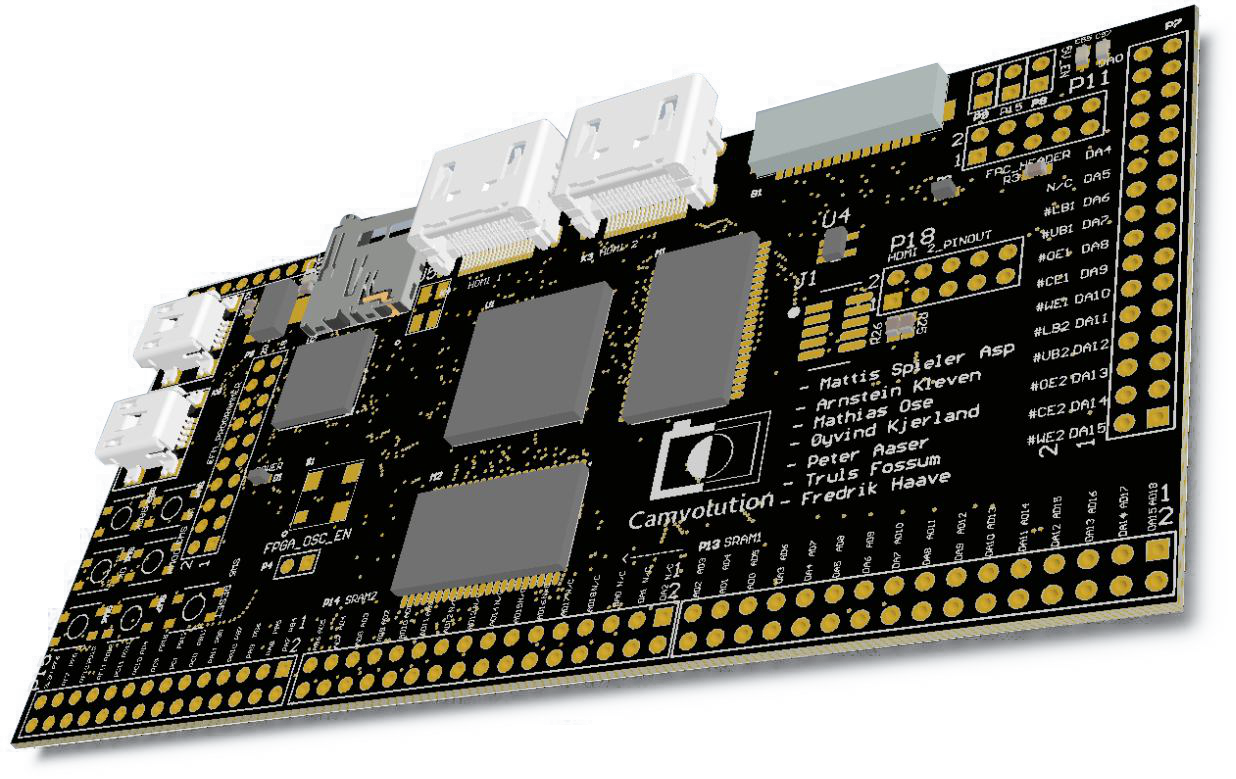
\includegraphics[width=\linewidth]{img/OverviewCamvolutionKit}
    \caption{Camvolution board layout}
\end{figure}

\subsection{Features}
\begin{itemize}
    \item Xilinx Spartan 6 FPGA
    \item Giant Gecko 990 EFM
    \item Connectors
        \begin{itemize}
            \item HDMI I/O
            \item FPC Camera
            \item MicroSD
        \end{itemize}
    \item 120MHz Oscillator for FPGA
    \item 48MHz Crystal for EFM
    \item Digital I/O
        \begin{itemize}
            \item 7 Mechanical Buttons
            \item 7 Expansion Headers
            \item 2 LED's
        \end{itemize}
    \item External memory
        \begin{itemize}
            \item 2 AS7C38098A SRAM
        \end{itemize}
\end{itemize}

\begin{figure}
    \includegraphics[width=\linewidth]{img/"Overview of Camvolution kit".jpg}
    \caption{Overview of Camvolution board}
    \label{fig:BoardLayout}
\end{figure}

\subsection{Power Supply}
The board is powered by a MiniUSB connector, with two possible options for powering it. Either connect it to the pc, or use an 5V USB power supply.

The 5V is regulated with a 3.3V LDO regulator, which gives power to most of the board.
This 3.3V is also connected to a 1.2V LDO regulator, that powers a minimum required power pins on the Xilinx Spartan 6 FPGA. 

\subsection{Clock Generation}
\subsubsection{FPGA Oscillator}The oscillator is connected to an enable signal on the EFM32 pin PF12.
To enable the 120MHz oscillator PF12 must be set to output and driven high.
The oscillator enable pin is also connected to an external input and can be set high by connecting this pin to VCC.
The easiest way of enabling the oscillator is to add a jumper on the FPGA\_OSC\_EN header.

\subsubsection{EFM External Crystal}
The EFM has internal and one external clock.
The external clock source is 48MHz and can be set by using the guide from the EFM, on how to enable external clock source.

\subsection{Connectors}
\subsubsection{HDMI}
There are two HDMI connectors on the board, both of them HDMI1 and HDMI 2 must also be connected to 5V, and can be set with a jumper at header 8, and header 15 respectively at the upper right corner.
The HDMI 2 is also connected to output pins at P18, this can be used for debugging.
Se table \ref{HDMI_Connector} in apendix for pinouts.

\subsubsection{FPC Raspberry Pi camera connector}
There is 1 Raspberry Pi camera connector on the board.
It is also connected to header P11, and can be used for debugging.
Se figure \ref{fig:FpcHeader} in apendix for pin configuration.

\subsection{Digital I/O}
\subsubsection{Buttons}
The board contains 7 buttons, and are all connected to pull-up resistors.
When the button is pushed down the input pin will be grounded.

The FPGA has 2 buttons for control.
These are connected to bank 1 on the P15, and P16 pin.
The MCU has 4 buttons for control.
These are connected to PD8, PD7, PD6 and PD5.
Se table \ref{tab:Buttons} n apendix for info.
The last buttons is connected to reset on EFM.

\subsubsection{Header output}
The EFM has spare pins that all are available on the P15 header pins.
Pin 28 on P15 header is 3.3V VCC.
The rest is pinouts from the EFM.
Se table \ref{tab:HeaderOut} in apendix for location of pins.

\subsection{SRAM}
\label{subsec:sram}
The FPGA is connected to two SRAM chips from Alliance Memory, one on bank 1 and another on bank 2.
They support a data width of 16 bits and have an access time of \unit[10]{ns} \cite{sramdatasheet}, which means we have a maximum throughput of $(\unit[10]{ns})^{-1} = \unit[1,6]{Gbps}$ to each chip.
This is more than sufficient for our application as can be seen in Table \ref{tab:BitRates}, but we do expect this number to be significantly less due to latencies introduced on the FPGA and by the wires in between.

To make debugging easier, all wires connecting the FPGA and SRAM chips have been placed on headers.

\subsection{JTAG and Programmer}
Both the FPGA and the EFM is connected with pinouts to a programmer.
The EFM is connected to a 20 pin header that can be used with the generic programming pin from a EFM development kit.
The FPGA is connected to a 8 pin JTAG header, this can be routed to a debugger used for FPGA programming.
See table \ref{tab:EfmProgrammer} for EFM programmer pin, see figure \ref{fig:FpgaProgrammer} for FPGA programmer pin.

Program\_B is connected to PB11, Done is connected to PB12.
\begin{table}[]
    \centering
    \begin{tabular}{ll}
        Pin                     & USAGE     \\
        \hline
        1                       & VCC       \\
        3                       & N/C       \\
        5                       & N/C       \\
        7                       & CS / PF0  \\
        9                       & CLK / PF1 \\
        11                      & N/C       \\
        13                      & PF2       \\
        15                      & RESET     \\
        17                      & N/C       \\
        19                      & N/C       \\
        4,6,8,10,12,14,16,18,20 & GND       \\
        2                       & N/C
    \end{tabular}
    \caption{Programming Output for EFM}
    \label{tab:EfmProgrammer}
\end{table}

\begin{figure}
    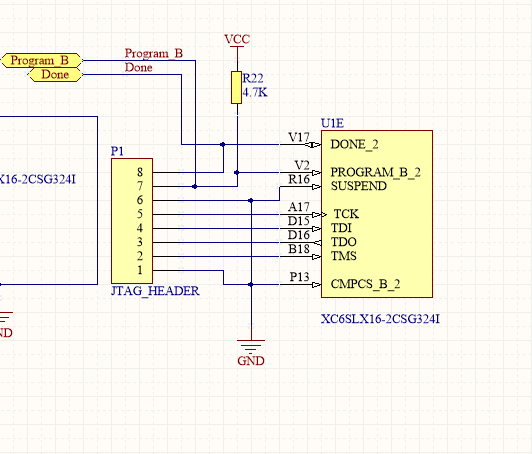
\includegraphics[width=\linewidth]{img/FPGA_Programmer}
    \caption{Programming output for FPGA}
    \label{fig:FpgaProgrammer}
\end{figure}

\subsection{Programming FPGA using EFM SPI}
The FPGA can also be programmed from the EFM using SPI from the EFM.

INIT\_B shares the same pin as the SRAM2 data line, but when programming the FPGA the SRAM will not be active.
Se table \ref{tab:SpiProgrammer}

\begin{table}[]
    \centering
    \begin{tabular}{lll}
        EFM pin & FPGA & Usage   \\
        \hline
        PB8     & U3   & INIT\_B \\
        PD3     & U15  & CS      \\
        PD2     & R15  & CLK     \\
        PD1     & V16  & RX      \\
        PD0     & R13  & TX
    \end{tabular}
    \caption{Programming FPGA using EFM SPI}
    \label{tab:SpiProgrammer}
\end{table}

\subsection{LED}
There are 2 LEDs on the board.
One is connected to power on the board and will light up if power is connected.
The last LED is programmable from the FPGA on pin N11.
Set this pin high and the LED wil light up.

\subsection{EBI-BUS}
The FPGA and the EFM is connected with a high speed parallel bus.
20 addressable pins and 16 data lines.
Se figure \ref{fig:EbiBus} and \ref{fig:EbiControl} for EFM pins.
Both figures are found in apendix.

There has been one change in the layout, the EBI\_WEn pin as shown in figur \ref{fig:EbiControl} is connnected to U10 instead of J6.

\subsection{Design faults}
In this 1\textsuperscript{}st revision fo the pcb, we made a few design faults that we had to make small hacks to fix.

\subsubsection{Voltage regulator}
Our first encounter was the voltage regulator that was connected to ground, but through a 100 ohm resistor and a capacitor.
This forced the voltage output up to 4.15v and may have bricked our fpga that has a voltage maximum at 3.95v.
The reason for this flaw was a failure to read the full specs of the datasheet.

\subsubsection{Memory card}
After mounting the SdCard-connector we found that all the pinouts on the sdcard was inverted.
The easiest solution was to the turn the SdCard-connector 180 degrees and mount part of it outside the board.
This was an acceptable fix for the mcu team.

\subsubsection{MCU clock48mhz}
There was a fail in the design of the 48mhz external clock pads for the MCU, this was due to failure of wiring the pads to the right pins on the external crystal.
To fix this we bought a new type of crystall, that had a smaller surface, and only two pins.
This flaw could have been avoided if we had printed out the pcb board on a A4 sheet, and tested the component fit on the pcb.
Unfortunatly we did not have the components at the time of ordering the pcb.

\subsubsection{Decoupling Capacitors}
Because we used a 0603 footprint for capacitors and resistors.
We then had to change to a bigger 0805 or 1208 footprint when mounting a capacitor larger then 10uF.
This is because capasitors at this many uF does not exist in 0603 footprint.
In the heat of the last few days, the pcb team forgot about this and we do not have 100uF capacitors decoupling on the pcb.

\subsubsection{HDMI connector}
At the time of routing the HDMI connectors to the fpga, we had no plan to use the HDMI as input for video.
Still we made an extra HDMI connector in case one should fail.

\paragraph{GCKLOCK problems on input}
Because of later problems with the rpi camera we had to look for other input solutions.
Unforturnatly the HDMI input clock $+$/$-$ needs to be connected to G\_CKLOCK pins on FPGA.
And we had only connected TDMS 0/1/2 $+$/$-$ to G\_CLOCK.
Because this wireing is impossible to change afterwards, we opened the HDMI cable and switched the cables internal pins to make it work.
This error only exist when using HDMI as input, and therefore we where not aware of this at the early time of pcb design.

\paragraph{Data communication between devices}
The HDMI has also a I2C interface, that it uses to communicate its display data.
Such as supported devices, monitor parameters etc.
This is not required for HDMI to actually work, but on most computers the HDMI will not output anything unless you force output HDMI signals, or send in this display data.
To make this job easier we could have added some routing to the I2C cables connectors on the HDMI connector.
// link to wiki https://en.wikipedia.org/wiki/Display\_Data\_Channel.

\subsubsection{Comments on design faults}
The amount of design faults on this board is not that many, the few we had was not that difficult to make workarounds for.
If we could make a second revision of the board, we would fix the design faults.
Add more leds, to make it easier for debugging.
And support a USB interface to the computer.
This could have been done with a extra small microcontroller that enables flashing of the Silent Gecko.

\subsubsection{List of components}
Se table \ref{listofcomponents} in apendix for a list of components used on the board.

